\section{Device}
\label{sec:device}

\subsection{Sensor Suite}
\begin{figure*}[t]
    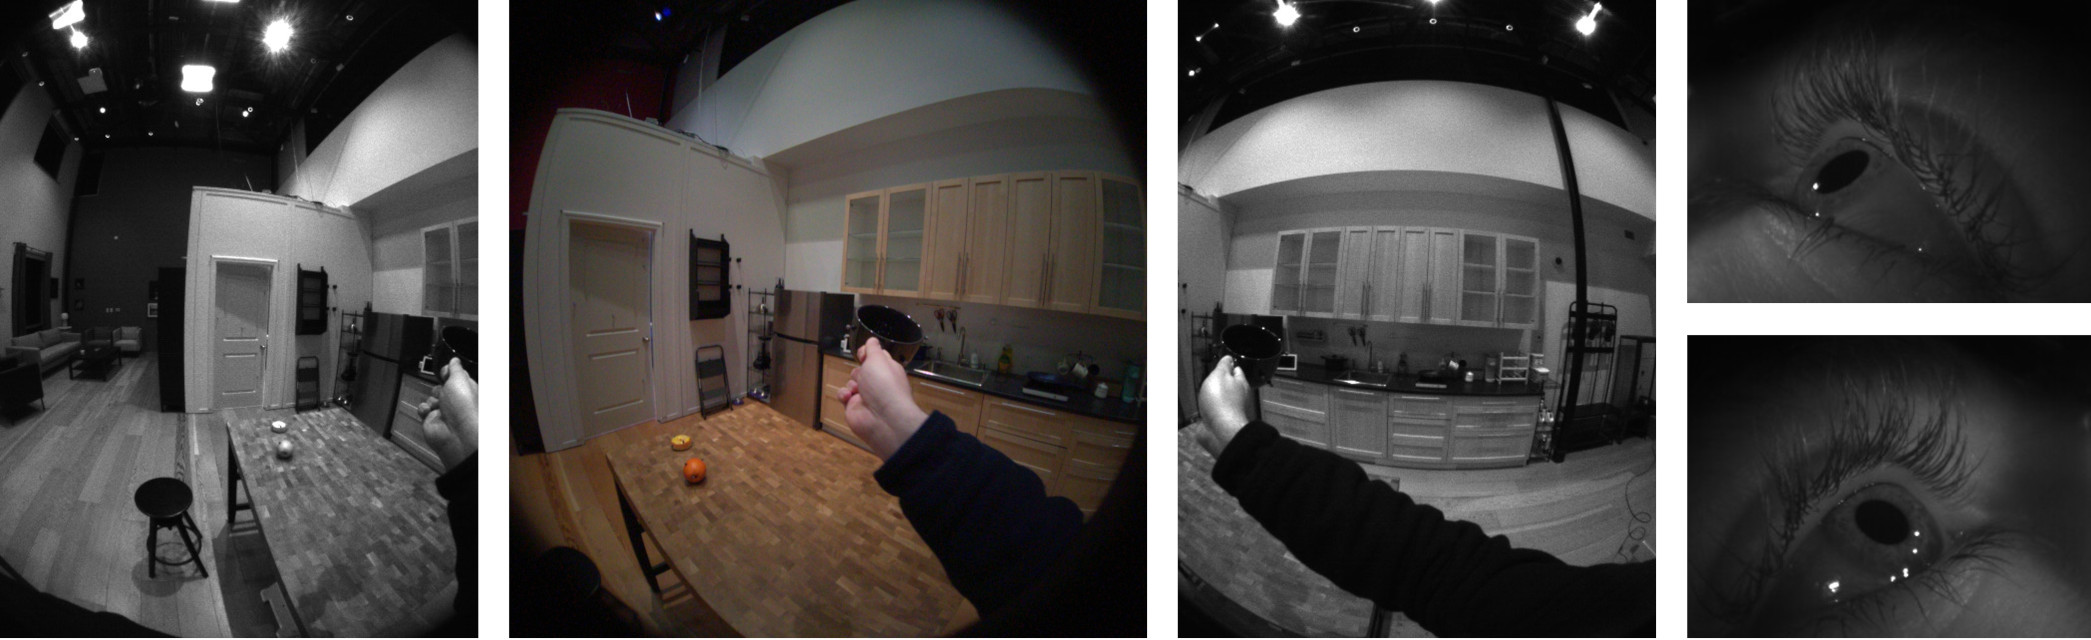
\includegraphics[width=\linewidth]{images/sampledata/CameraSampleImages.jpg}
    \caption{Example images from the \AriaDevice{} cameras. Left to right: left Mono Scene camera, POV (RGB) camera, right Mono Scene camera, two Eye-tracking cameras. Output of POV (RGB) and Mono Scene cameras are rotated for visualization.}
    \label{fig:aria-multi-modal-scene-cameras}
\end{figure*}


We built the \AriaDevice{} to emulate future wearable devices catering to machine perception rather than human consumption. To mimic the sensor stack needed for machine perception capabilities on these future devices, we integrate a rich suite of sensors that record egocentric multi-modal data (see 
Figures~\ref{fig:aria-multi-modal-scene-cameras}\,--\,\ref{fig:aria-multi-modal-gps-wps}).

Sensor streams are tightly calibrated and time-aligned to make some problems fundamentally easier to solve.  This is aligned to future expectations of wearable device hardware, but introduces new challenges - such as the lack of Optical Image Stabilization (OIS) or Auto-Focus (AF). 

To satisfy the strict requirements for capturing representative data in a wearable form-factor constraints, we built the \AriaDevice{} as a data-collection and streaming device. Specifically, it is not designed to handle on-device computation workloads.


\subsection{Form Factor and Fit}
The \AriaDevice{} is designed to contain a rich set of sensors while being light (around 75g) and socially acceptable. The devices provide a good fit for a broad range of the population with two device sizes. They come with adjustable nose pads and temples (i.e.~the temple tips can be bent inwards or outwards to improve fit). The glasses temple have a lot more flexibility than a conventional pair of glasses, which means the small size can stretch up to what many glasses might call a medium or large size. 


The sensors on the \AriaDevice{} have been chosen to (1) approximate what we expect to be available on future all-day-wearable AR glasses, and (2) fit into the strict size, weight and power envelope required by the target form-factor to obtain ecologically valid data. We selected a broad range of sensors beyond just cameras as we believe multi-modal egocentric data to be key to solve various Machine Perception and AI tasks -- see Section~\ref{sec:applications} for some examples. The following gives an overview of what sensors are available on a \AriaDevice\ (see also Figure \ref{fig:aria-glasses-blowup}):
\begin{itemize}
  \setlength\itemsep{0em}
\item \textbf{Mono Scene Cameras}: Two monochrome, global-shutter cameras on the left and right side of the glasses. They have a horizontal field of view (HFOV) of 150\textdegree\ and are angled outwards to maximize peripheral vision while allowing for some stereo overlap. These cameras are used for supporting machine perception capabilities such as Visual SLAM~\cite{engel2014lsd, mur2017orb, mourikis2007multi}.
They have a resolution of 640x480 pixels and use Fisheye (F-Theta) lenses.
\item \textbf{Point of View (POV) RGB Camera}: A single high-resolution, rolling-shutter RGB camera on the left side of the glasses with a HFOV of 110\textdegree. The RGB camera also uses a F-Theta Fisheye lens, has a maximum resolution of 2880x2880 pixels and faces forward with an approximately 4\textdegree\ bias towards the ground. 
\item \textbf{Eye Tracking Cameras}: Two monochrome, global-shutter, inward-facing cameras for eye tracking with a diagonal field of view (DFOV) of 80\textdegree. They typically operate at a 320x240 pixels resolution.
\item \textbf{IMUs}: Two inertial measurement units (IMU), one on each side of the glasses. The left IMU is configured to sample at 800\,Hz with saturation limits of 4g (accelerometer) and  500\textdegree/s (gyroscope). The right IMU samples at 1000\,Hz with saturation limits of 8g and 1000\textdegree/s. We intentionally chose different IMU models so that their higher-order error behaviors are more likely to be uncorrelated.
\item \textbf{Microphones}: A microphone array comprised of 7~microphones distributed around the glasses (5 front, 1 on each side), allowing to capture spatial audio at 24\,bits with a configurable sample rate of up to 48\,kHz.
\item \textbf{Magnetometer}: A magnetometer located on the rim of the glasses to minimize electromagnetic interference, measuring the ambient magnetic field (3-axis) with a resolution of 0.1\,$\mu$T and a sample rate of 10\,Hz.
\item \textbf{Barometer \& Thermometer}: A barometer sensor capturing local air pressure and temperature at a resolution of 0.66\,Pa and 0.005\textdegree\,C, respectively, with a sample rate of 50\,Hz.
\item \textbf{GNSS receiver}: A global navigation satellite system receiver supporting GPS and Galileo constellations, providing pseudo-range measurements as well as lat/long/height solutions with a sample rate of 1\,Hz.
\item \textbf{Wi-Fi \& Bluetooth transceiver}: A Wi-Fi and Bluetooth radio with the ability to regularly scan and record received signal strengths (RSSI) from Wi-Fi beacon frames (both 2.4G and 5G) and from Bluetooth beacons. Scanning is nominally performed at 0.1\,Hz.
\end{itemize}

\begin{figure}
    \centering
    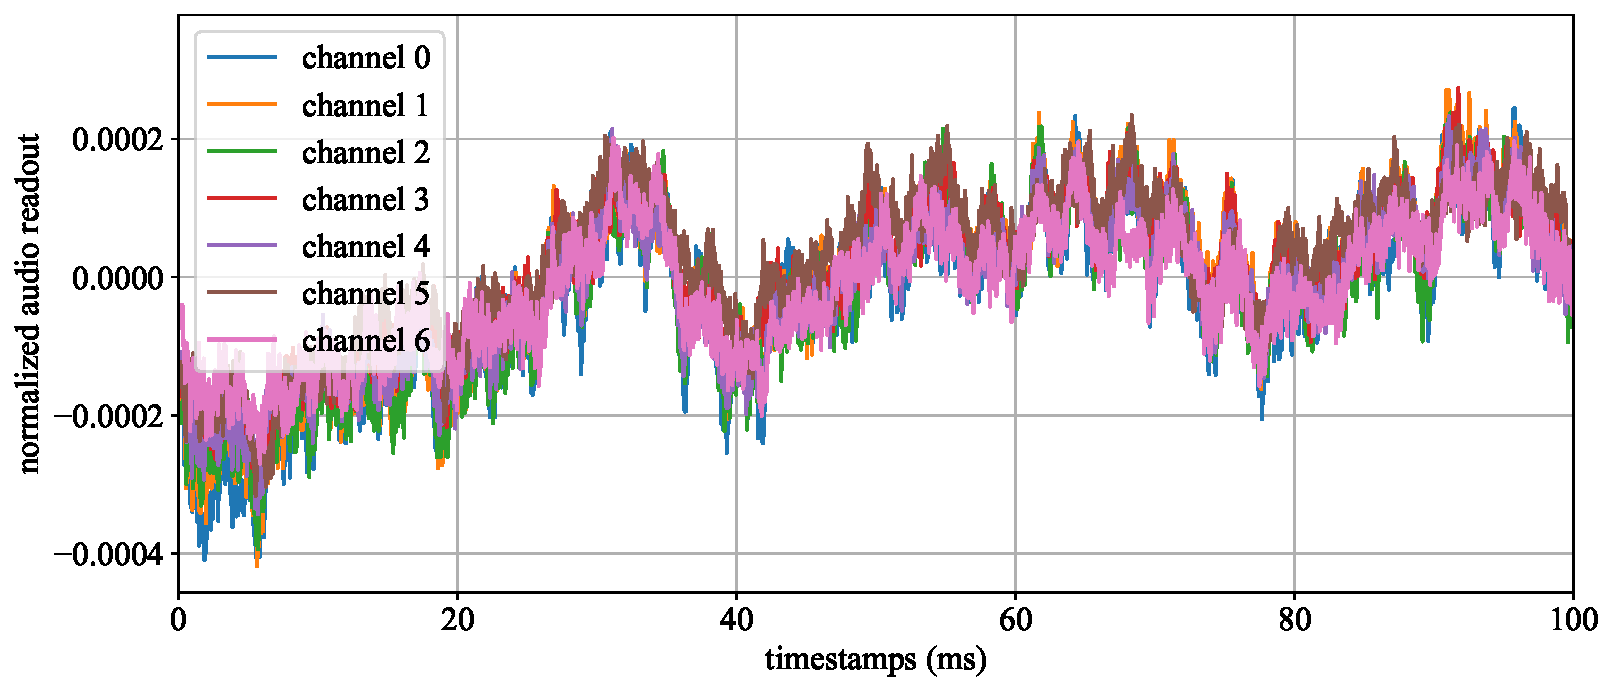
\includegraphics[width=\linewidth]{images/sampledata/audio_normalized.pdf}
    \caption{Example time-series data from the multi-channel microphone array on the \AriaDevice{}. Audio data is saved in 32-bit format and normalized in the range of $[-1, 1]$.}
    \label{fig:aria-multi-modal-audio}
\end{figure}


\begin{figure}[t]
    \centering
    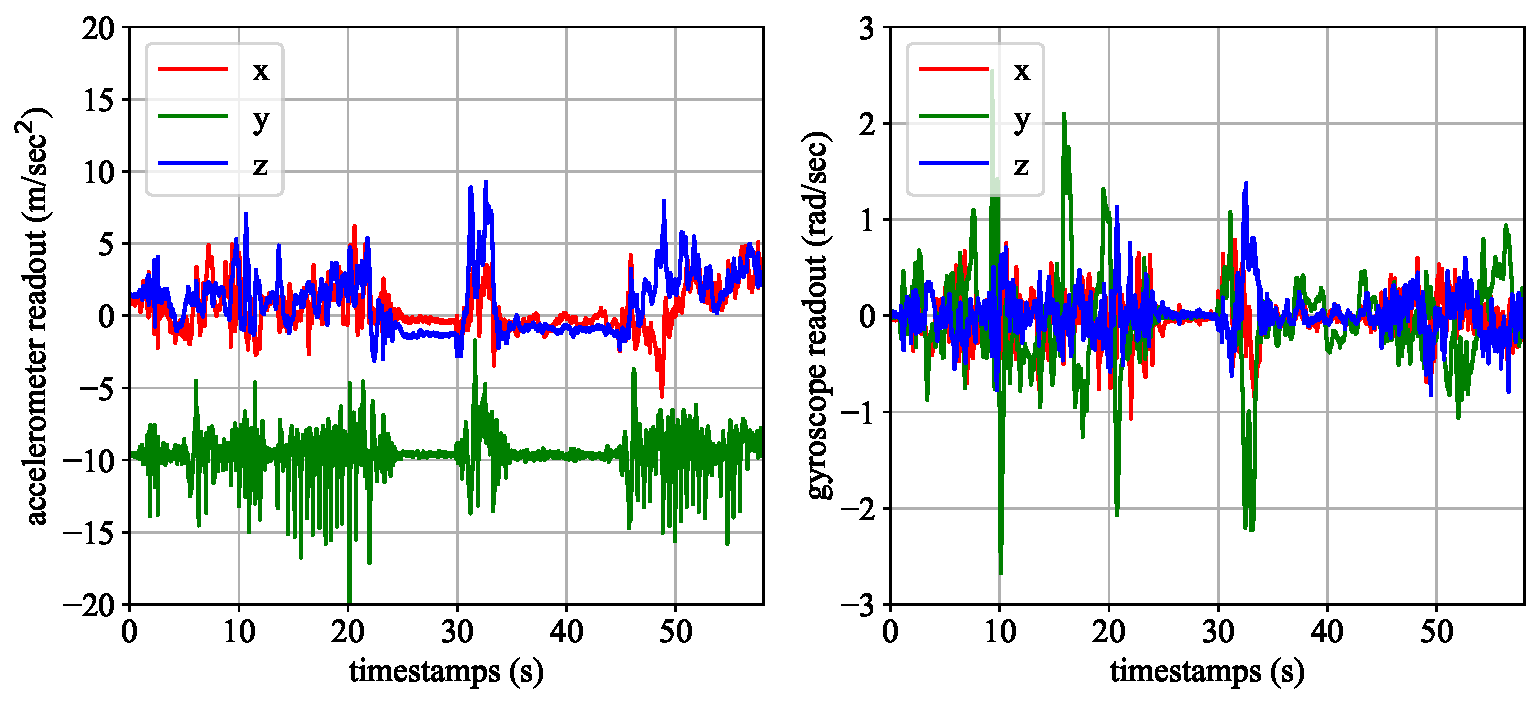
\includegraphics[width=\linewidth]{images/sampledata/imu.pdf}
    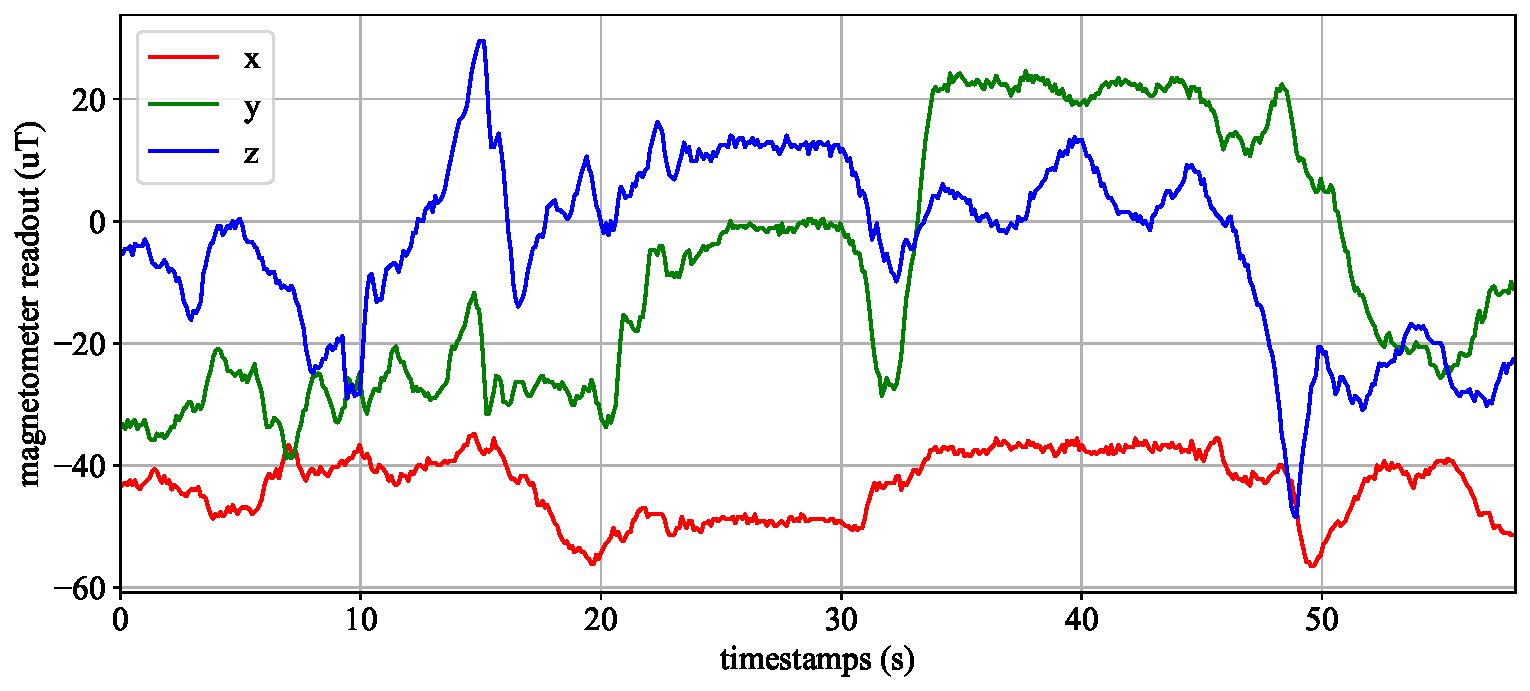
\includegraphics[width=\linewidth]{images/sampledata/mag.pdf}
    \caption{Example data from various motion sensor and location signal data. Top to bottom: accelerometer and gyroscope data provided by the IMUs, and magnetic field measurements provided by the magnetometer.}
    \label{fig:aria-multi-modal-data-imu-mag-baro}
\end{figure}

\begin{figure}[t]
    \centering
    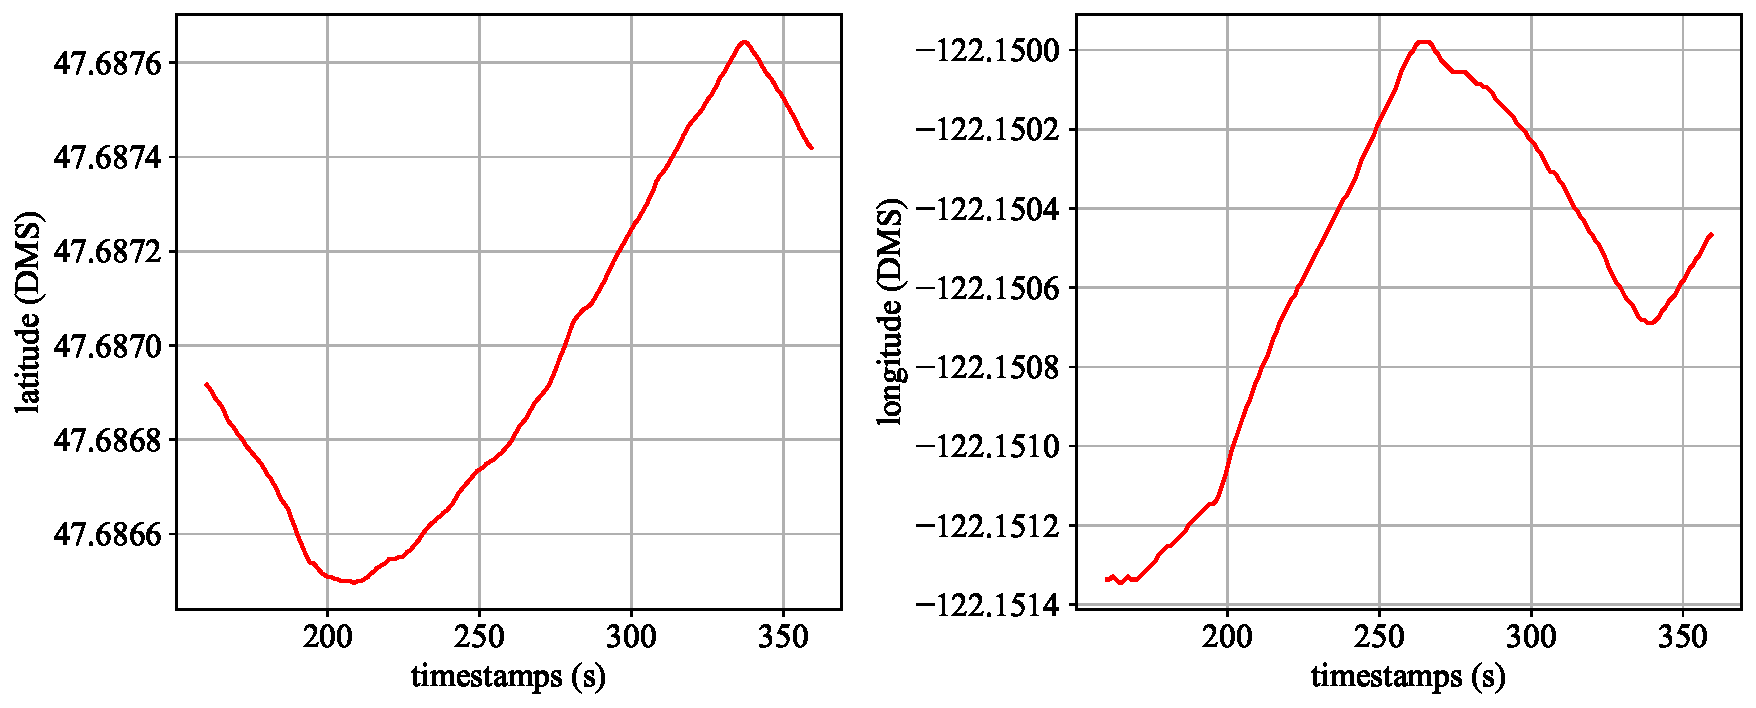
\includegraphics[width=\linewidth]{images/sampledata/gps.pdf}
    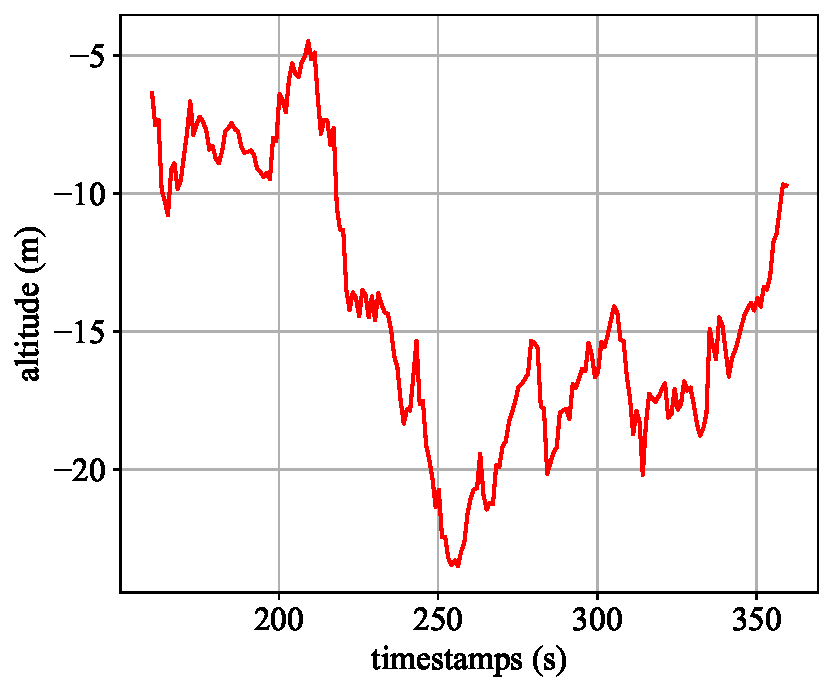
\includegraphics[width=0.49\linewidth]{images/sampledata/gps_altitude.pdf}
    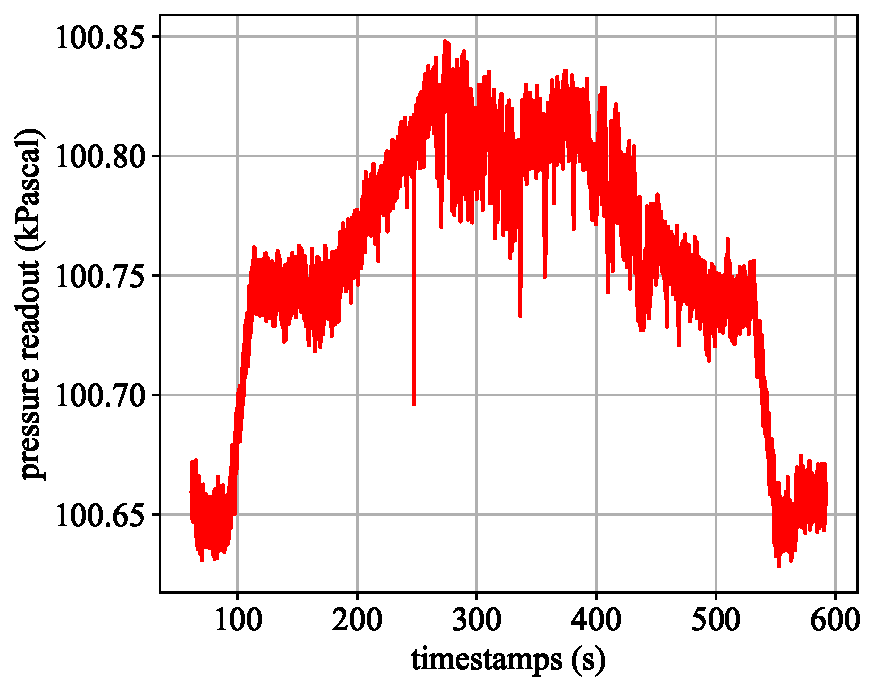
\includegraphics[width=0.49\linewidth]{images/sampledata/baro.pdf}
    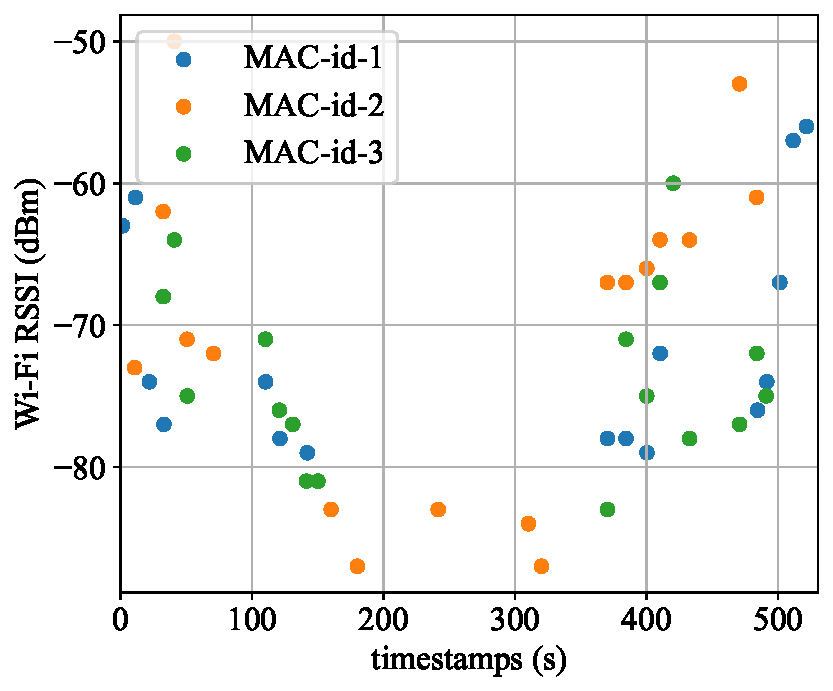
\includegraphics[width=0.49\linewidth]{images/sampledata/wifi.pdf}
    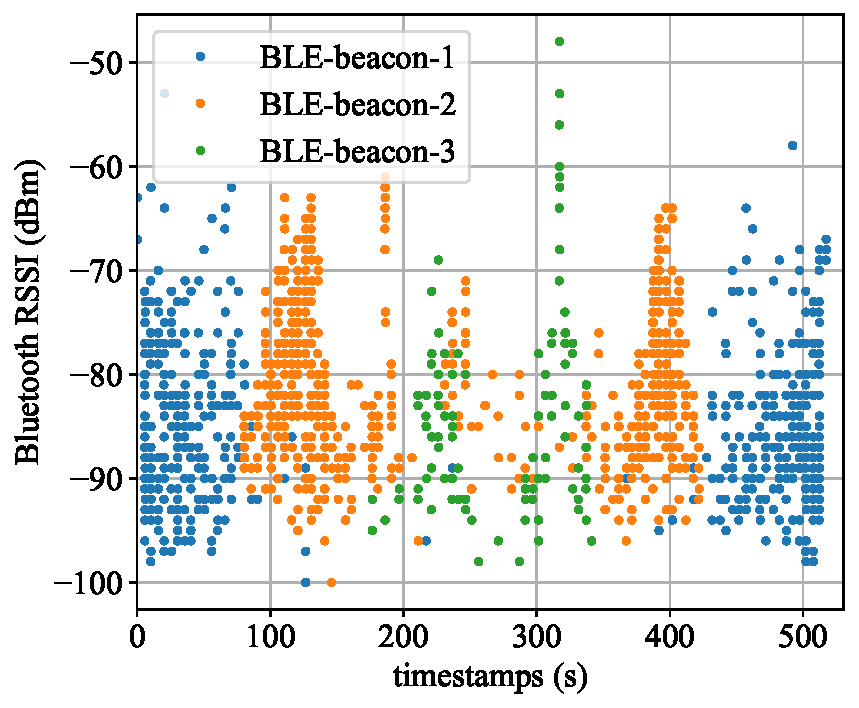
\includegraphics[width=0.49\linewidth]{images/sampledata/ble.pdf}
    \caption{Illustration of the GNSS and Wi-Fi/Bluetooth sensor data. Top to bottom:  GNSS signal (individual plots of latitude, longitude, altitude), pressure measurements provided by the barometer,
    signal strengths from different sources as recorded by the Wi-Fi and Bluetooth receivers. 
    }
    \label{fig:aria-multi-modal-gps-wps}
\end{figure}

Many of these sensor settings can be configured through \textit{recording profiles} that are selected at the start of a recording and allow to modify camera frame-rate and resolution, as well as to enable or disable different sensor streams. This is important as recording all sensors at maximum resolution and rate is not feasible due to power and bandwidth limitations. Furthermore, disabling sensor streams or reducing their rate and/or resolution can be desirable from a privacy perspective, and is an effective strategy to prolong maximum recording time. Available recording profiles are listed in the  \ProjectAria{} documentation site \cite{ariadocs}.


\subsection{Mounting and Rigidity}
Precise 6DoF alignment -- that is, relative positioning and orientation between all sensors -- is important for many basic machine perception algorithms, and the \AriaDevice{} has been designed to facilitate this. All sensors are mounted onto a magnesium frame spanning the front of the glasses. With the most non-rigid portion being the nose-bridge, there are two primary sensor clusters on the left and right side of the glasses. Sensors within the same cluster have a strong rigid connection.

We provide extrinsic and intrinsic calibration parameters for each sensor computed at manufacturing time (factory calibration). Through our Machine Perception Services (MPS, see Section \ref{sec:mps}) we additionally make more accurate online-calibration parameters available that account for the small deformations/changes that might occur while wearing the glasses. Please refer to \cite{ariadocs} for more details.

\subsection{Time and Time-alignment}

The \AriaDevice\ is designed to allow accurate timestamping 
of all sensor data with respect to a local on-device time source. This is essential to combine different modalities in downstream machine perception tasks.

In addition, \AriaDevices{} provide the ability to align and convert local timestamps to a time domain shared across multiple devices. Accurately translating to a common time domain is critical when combining or comparing data from different sources and devices. 
In our sample datasets, we use SMPTE~LTC~timecode~\cite{smptet} to provide a common accurate time domain across multiple \AriaDevices{} (see Aria Pilot Dataset \cite{ariapilot}). For situations where lower accuracy is acceptable we have also implemented a methodology for sharing a common time domain over Wi-Fi leveraging the TicSync timing protocol~\cite{conf/icra/HarrisonN11}. For both methodologies, the inner working of the time sharing mechanism is handled at the device level. This means, from the perspective of a user of the data, every sensor reading simply includes a timestamp in the aligned time domain in addition to a timestamp in the local device time.
Please refer to the  \ProjectAria{} documentation \cite{ariadocs} for more details on the exact definition and conventions for time\-stamps of the different sensor modalities. 


\begin{figure*}[pt]
    \centering
    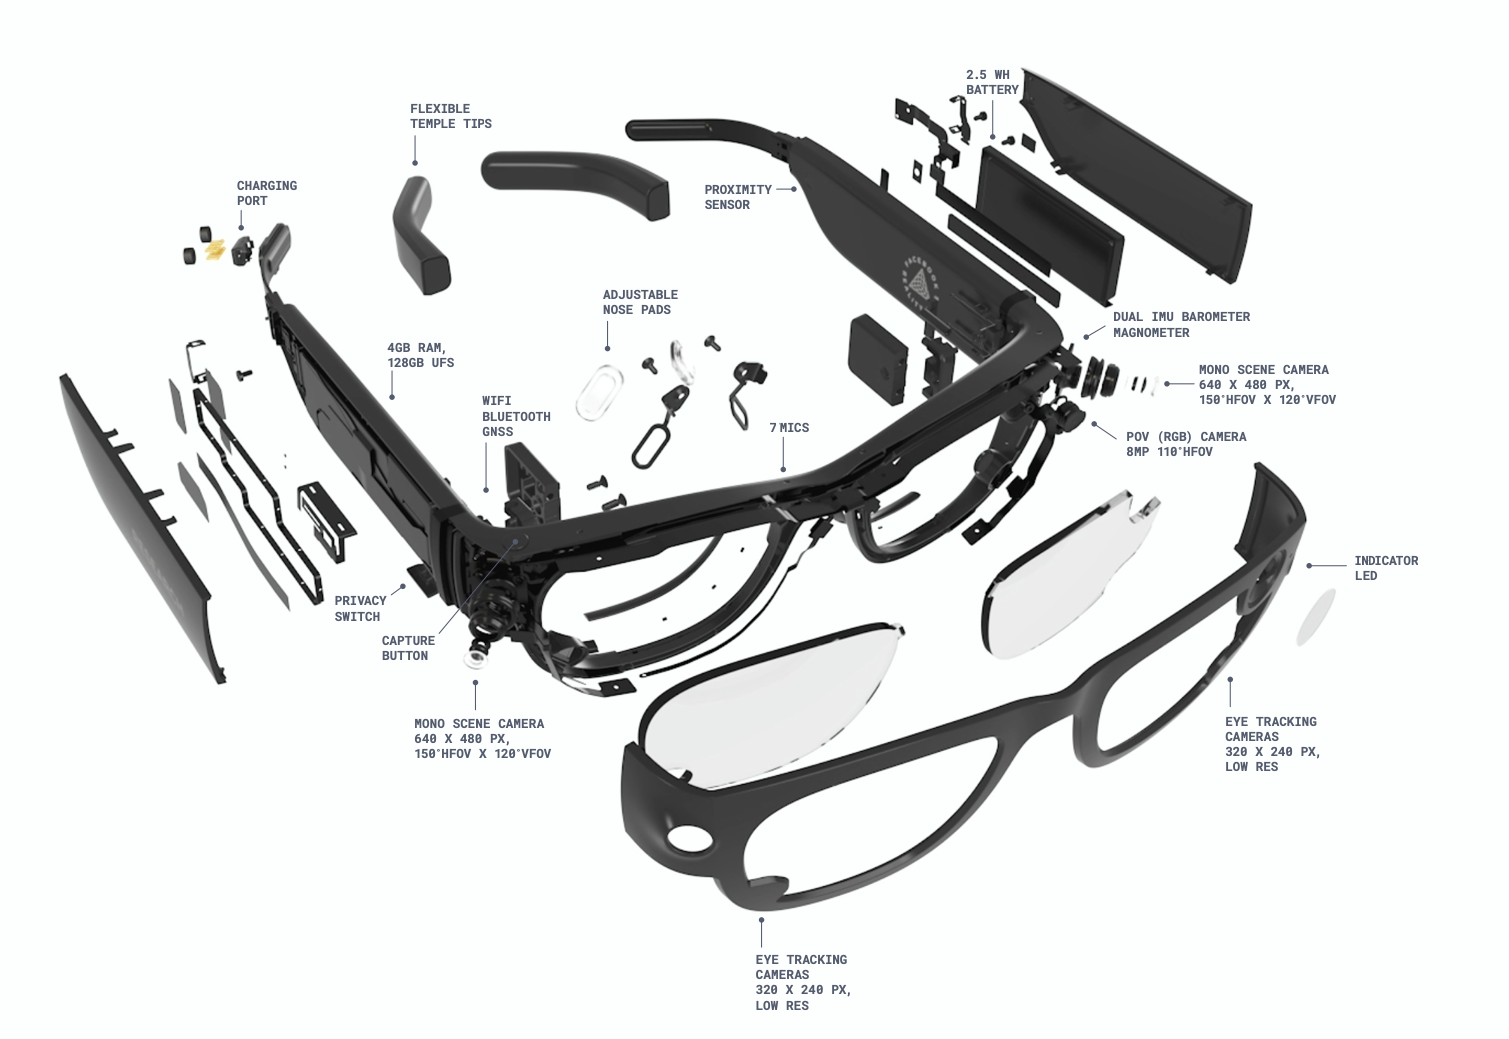
\includegraphics[width=0.95\linewidth]{images/aria_glasses_blowup2.png}
    \caption{\AriaDevice{} hardware overview of the components, the various sensors, switches, LEDs, battery, etc.}
    \label{fig:aria-glasses-blowup}
    \vspace{5mm}
\centering
    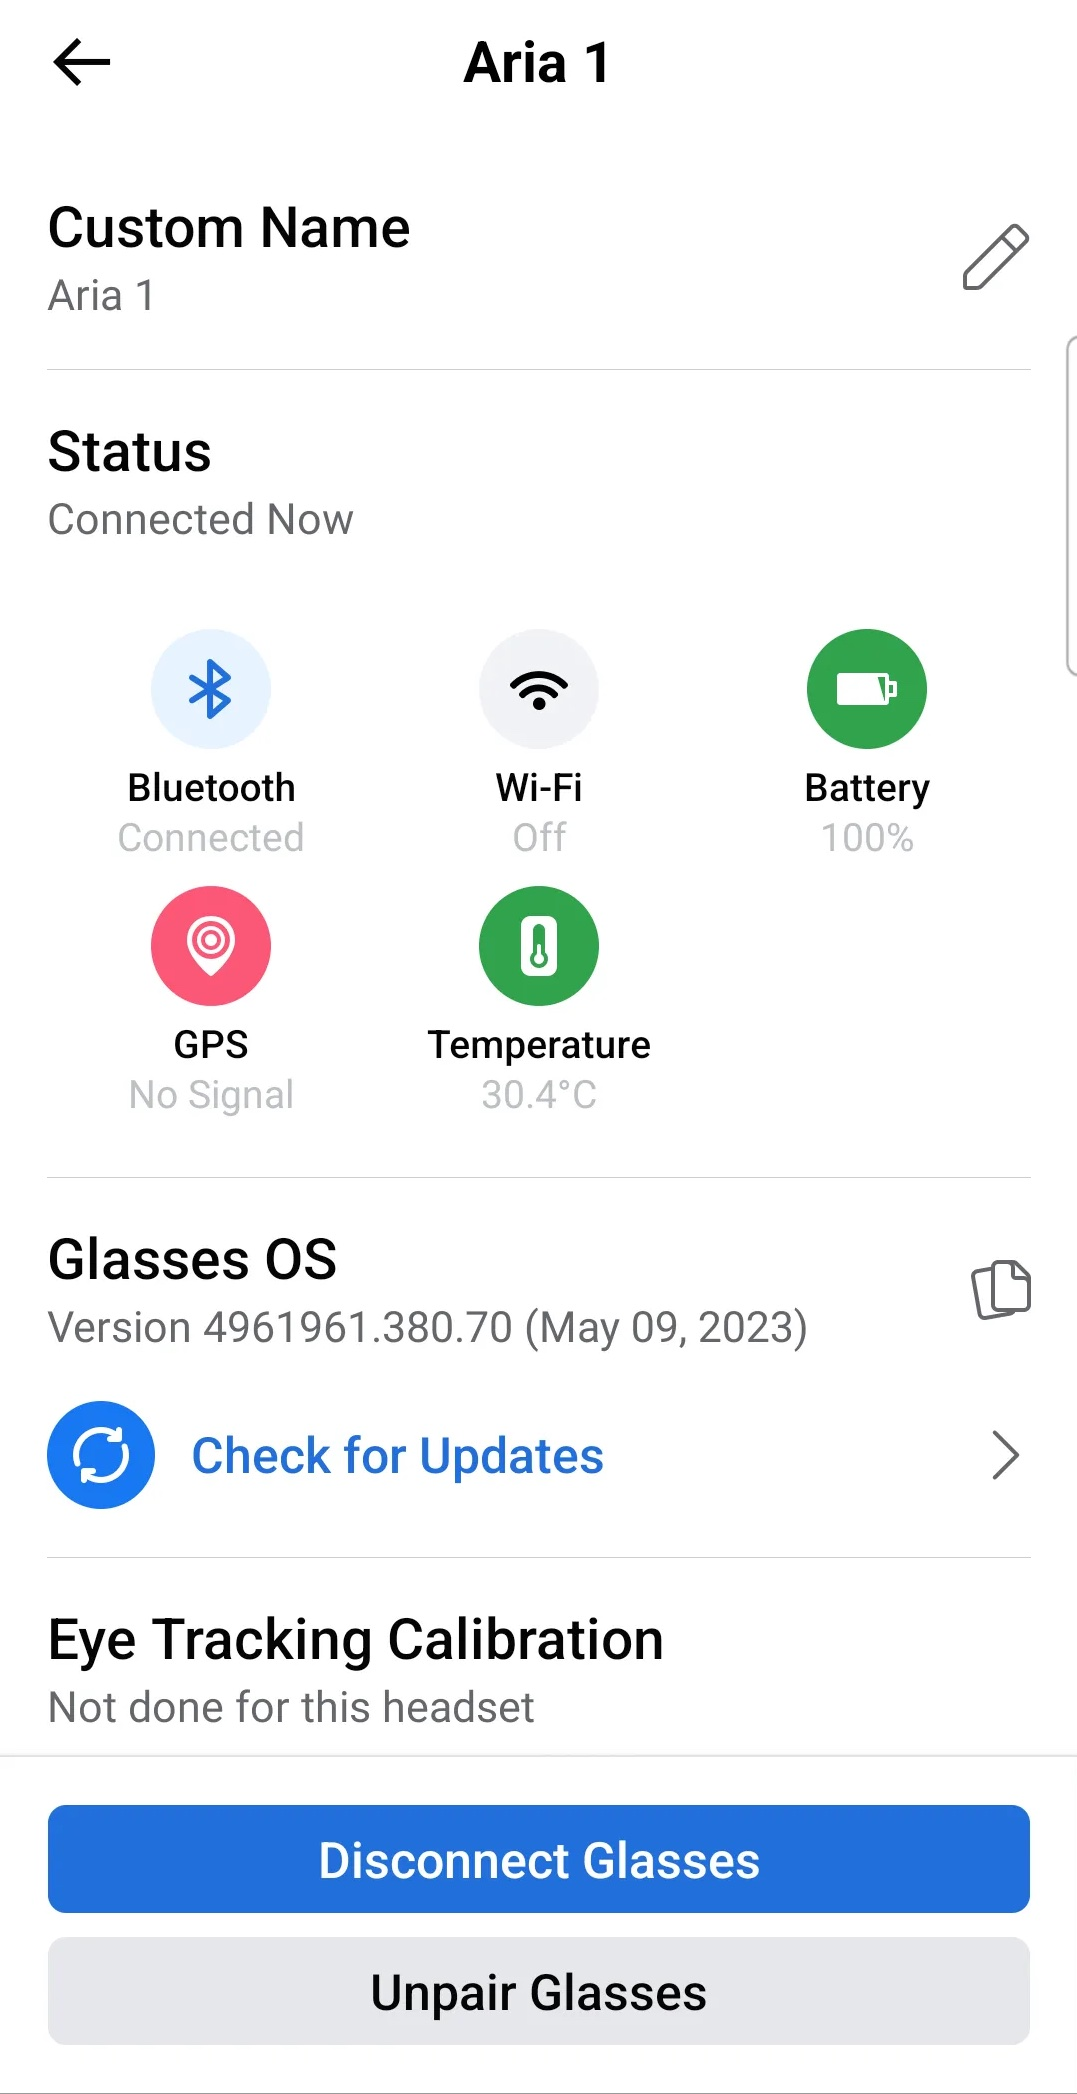
\includegraphics[frame,height=0.4663560112\linewidth]{images/companion_app/device_status.jpg}\hfill
    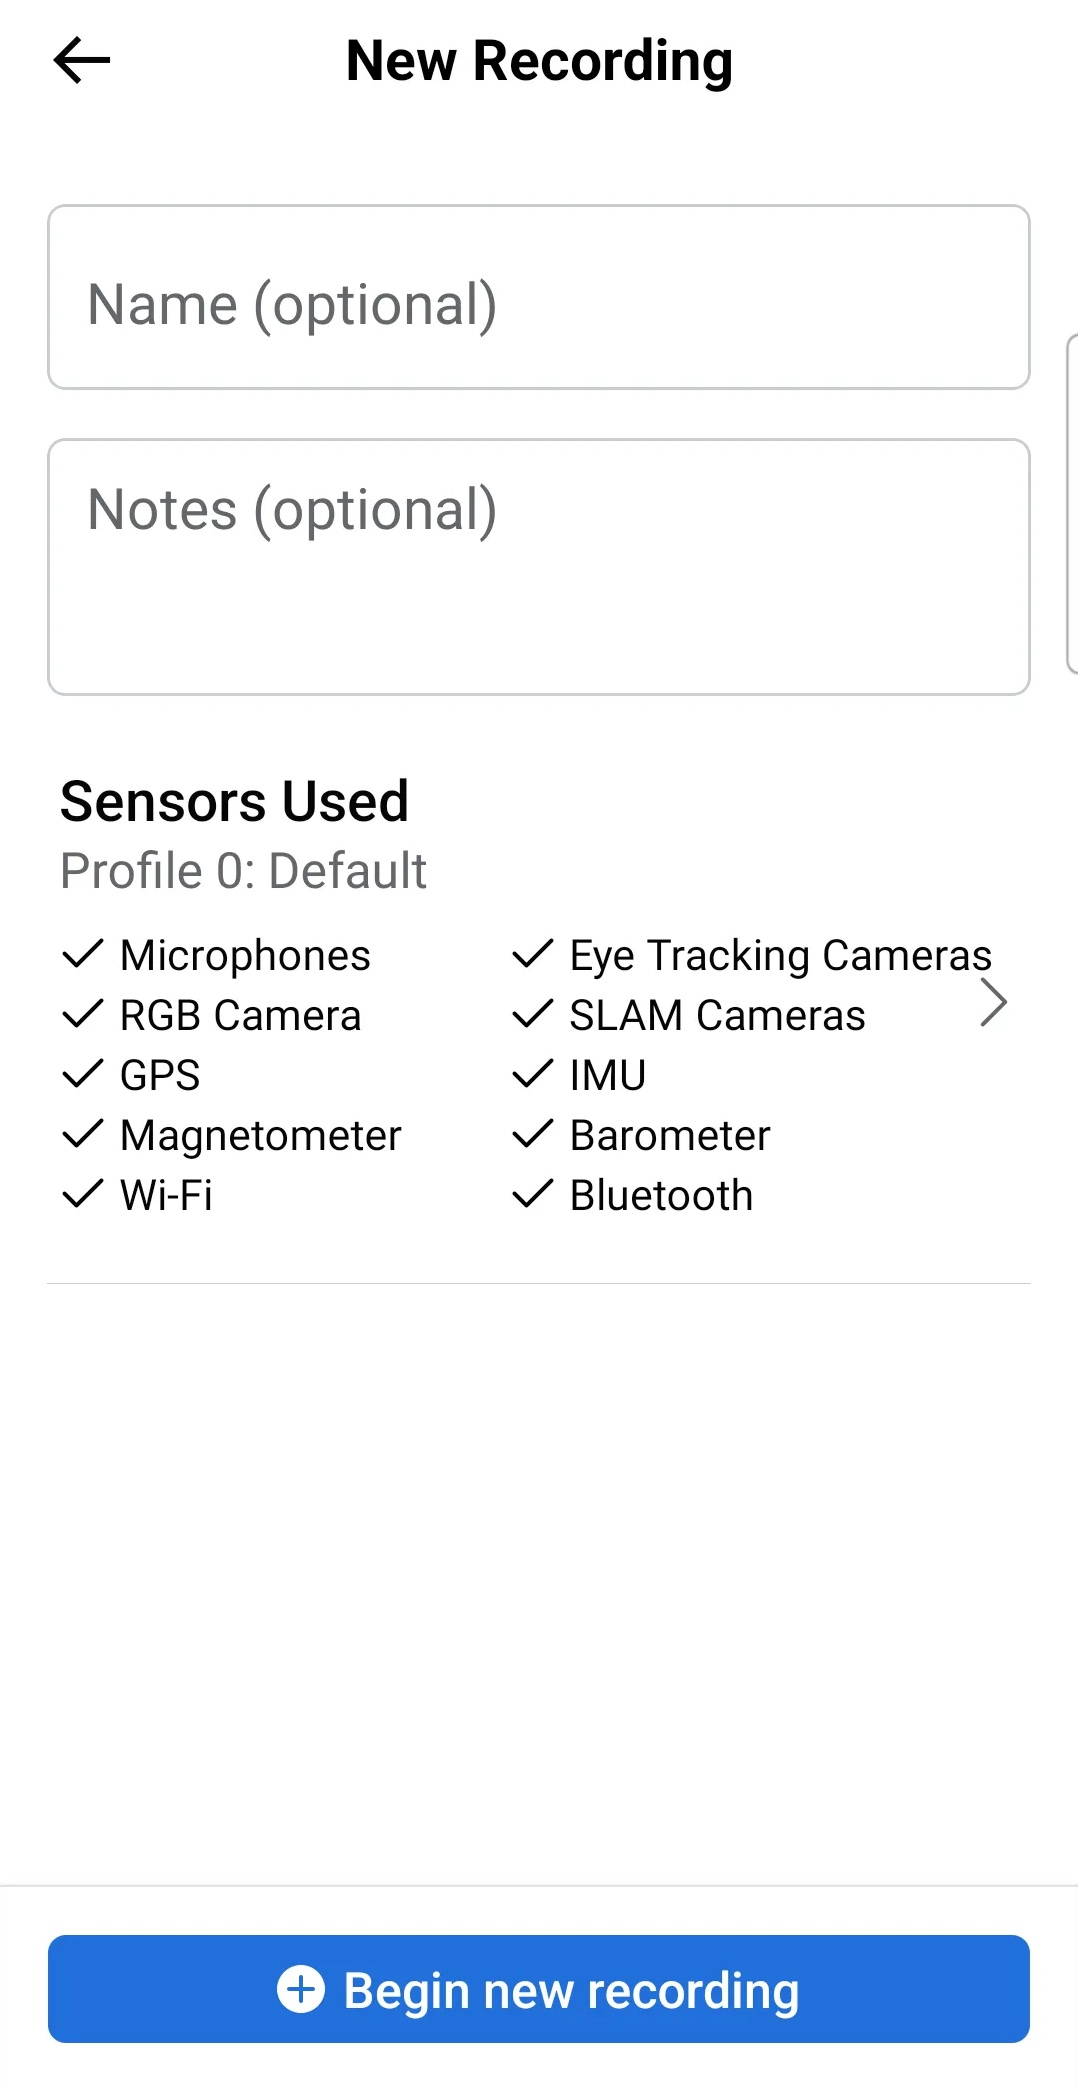
\includegraphics[frame,height=0.4663560112\linewidth]{images/companion_app/profile_selection.jpg}\hfill
    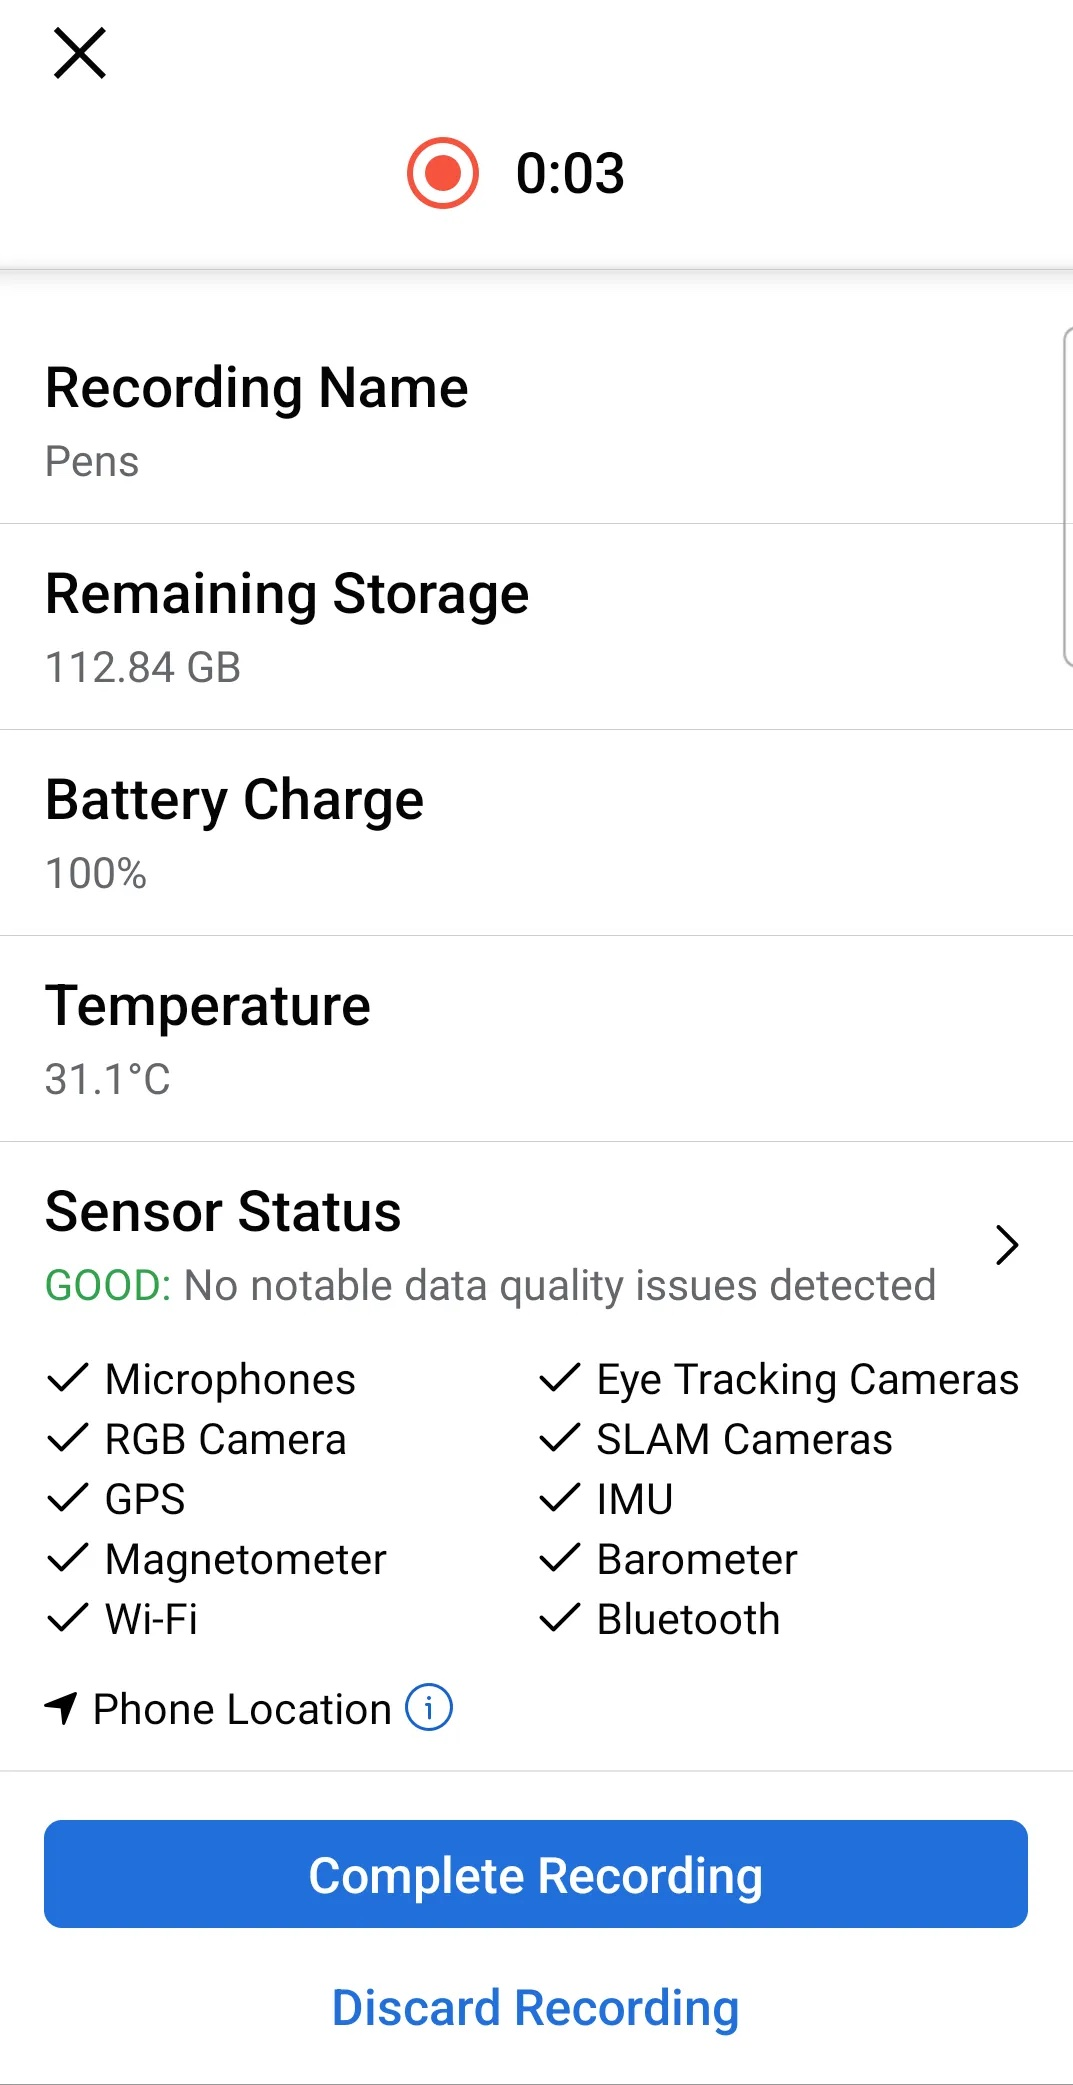
\includegraphics[frame,height=0.4663560112\linewidth]{images/companion_app/recording.jpg}\hfill
    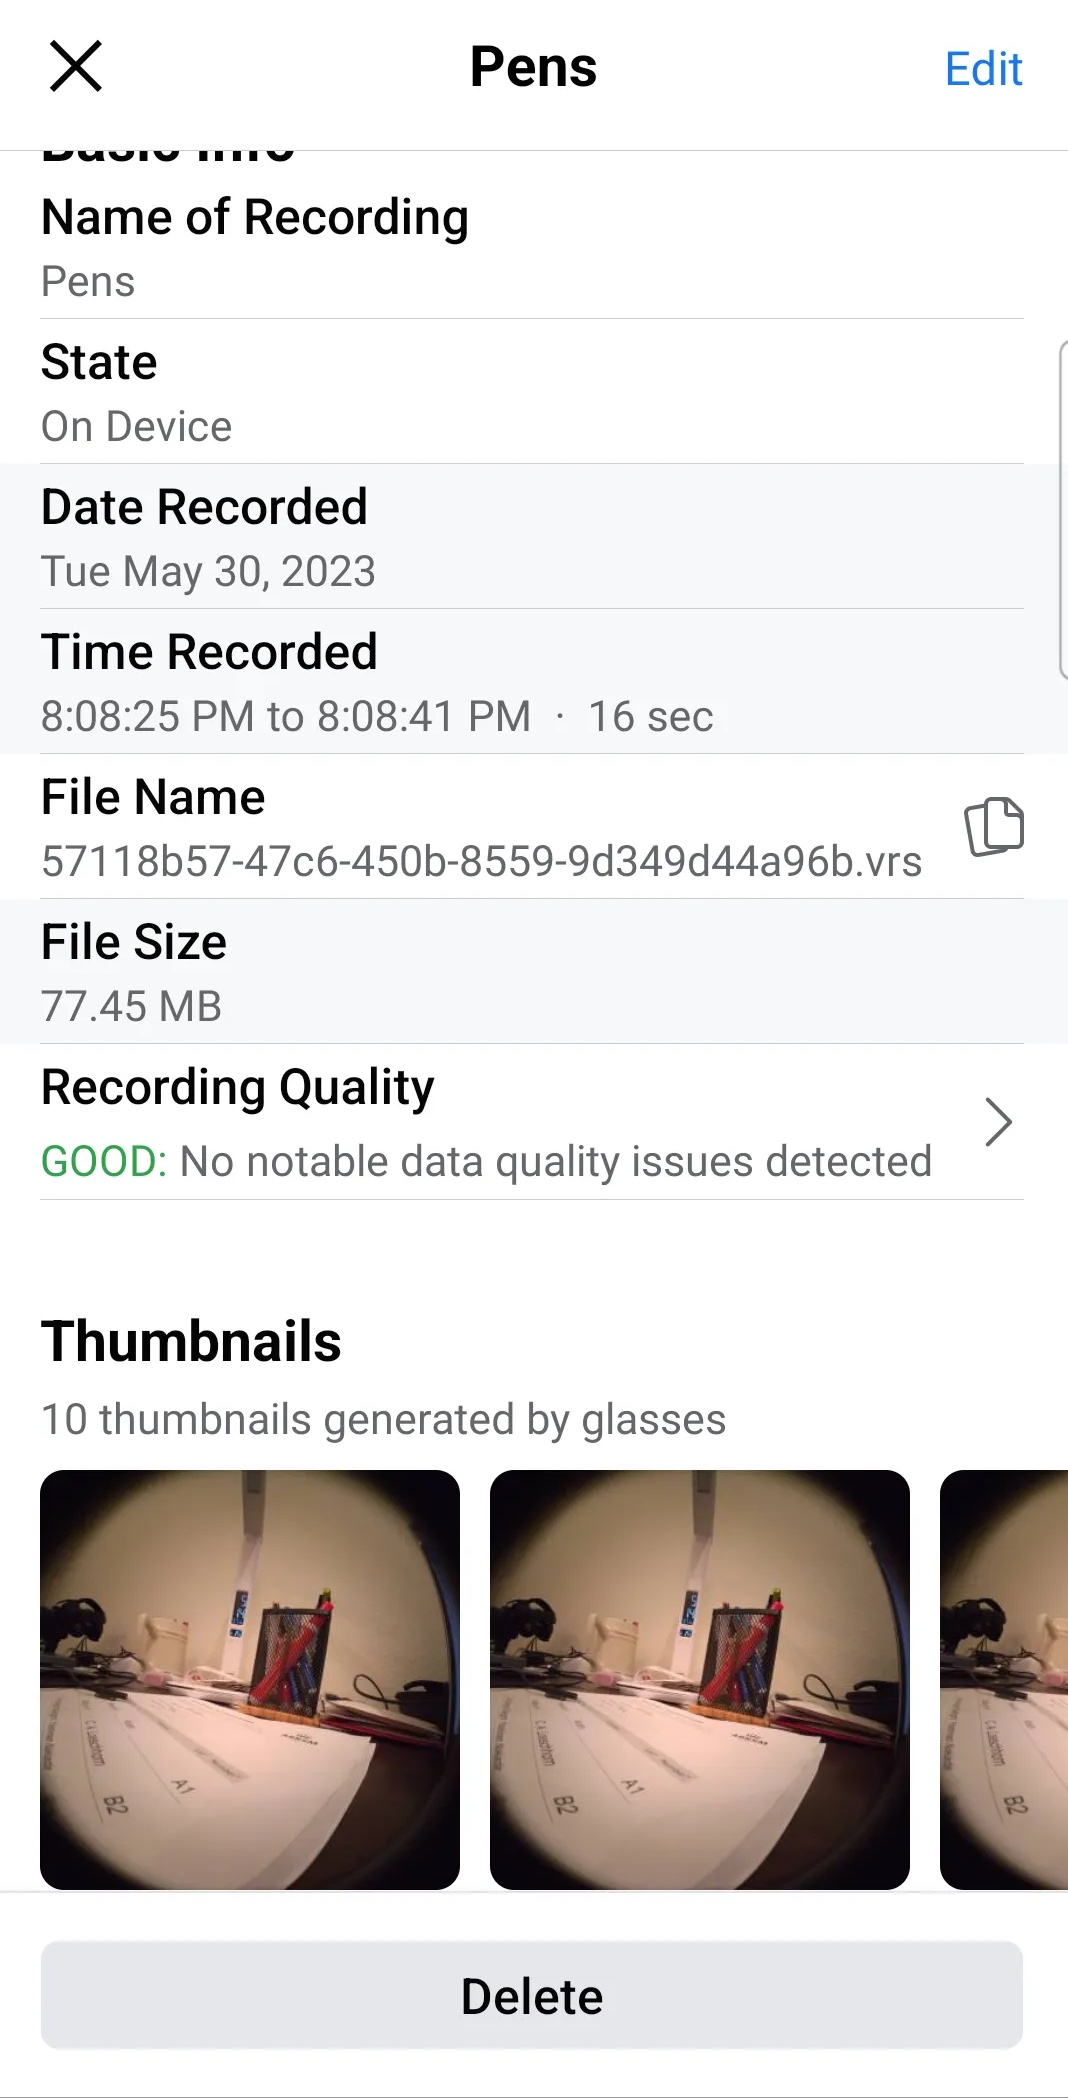
\includegraphics[frame,height=0.4663560112\linewidth]{images/companion_app/thumbnails.jpg}
    \caption{Basic functionalities of the mobile phone companion app. From left to right, the screenshots illustrate a) the device status information, b) the recording profile that configures the sensors before recording, c) status of the on-going recording, d) thumbnail preview of the recordings visible after a recording finishes}
    \label{fig:companion-app}
\end{figure*}

